\section{Offline Data Quality Monitoring}
\label{sec:monitoring}

Offline data quality monitoring (DQM) provides rapid feedback to the data-taking process. Offline computing should be aware of incoming data via the database stream within minutes of the start of a new run, triggering the first reconstruction pass (\passone, see section~\ref{sec:overview}). DQM code will run immediately afterward with access to all data streams to inspect tracks, calorimeter clusters, and all components of the system. The results should appear within a few hours of the start of a run, and experiment operations will have immediate access. DQM could be run at any other stage, including on raw data before \passone, during the calibration process, or on the final dataset production.

The first component of the system is histogramming. For simplicity and robustness, the system starts with histogramming the content of reconstruction output, but anything that can be computed in an art job can be reported. The output is a histogram file, labeled by the process which produced it, the run and subrun involved, and the degree of concatenation. Some quantities will require very little data to be useful, while some might need a full run or even many. An arbitrary level of concatenation is allowed. These histogram files are saved to disk for several weeks, then archived to tape.

The second step in the DQM process is to derive metrics from the histogram files, such as the mean or RMS of a histogram, the number of hits on a track, or normalized quantities (e.g. the number of CRV hits per time). These metrics are then labeled to keep track of the provenance, and inserted in the DQM database (see section~\ref{sec:databases}. The DQM core system (a nominal set of histograms and metrics) has been running for over a year as part of nightly validation.

The final part of DQM processing is displaying the results. Mu2e supports two display styles. The first is an overlay of histograms, for example, comparing the current run to the previous one or to a standard set of plots. Several tests of comparison are provided, including a systematic allowance. The second display style shows the metrics as a timeline, allowing for some selection on the display (see Figure~\ref{fig:timeline}). The system uses the ploytly package to allow interactive use.

Several standard sets of plots will be provided to the shift crew and experts, together with tolerances for histogram comparisons or acceptable ranges for the metrics. An alarm will be sent to experts when automatic comparisons are out of tolerance.

\begin{figure}[htb]
\begin{center}
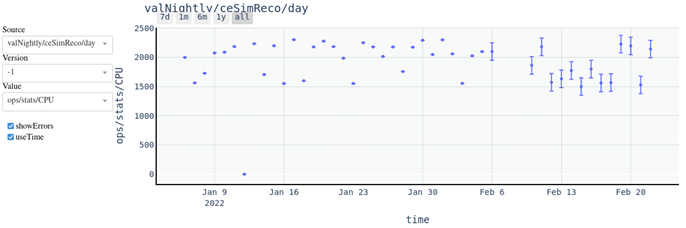
\includegraphics[width=0.9\linewidth]{figures/dqm_timeline.png}
\caption{An example display of a metric timeline}
\label{fig:timeline}
\end{center}
\end{figure}
